% !TeX spellcheck = en_US
\documentclass[a4paper, 11pt]{article}
\usepackage[utf8]{inputenc}
\usepackage{t1enc}
\usepackage[english]{babel}
\usepackage{lmodern}
\usepackage{url}
\usepackage{graphics}
\usepackage{listings}
\usepackage[a4paper, total={5.5in, 8in}]{geometry}

\hyphenation{UPPAAL}
\sloppy

\begin{document}
	
	\newcommand{\specialcell}[2][c]{%
		\begin{tabular}[#1]{@{}c@{}}#2\end{tabular}}
	
	\newenvironment*{mytable}[3]{
		% #1: caption, #2: cimke, #3: oszlopdef		 
		\begin{table}[htbp]	
			\caption{#1}          
			\label{tab:#2}            
			\center%
			\begin{tabular}{#3}
			}
			{
			\end{tabular}
		\end{table}
	}
	
	\pagestyle{plain}
	
	
	
	% angol környezet beállítása
	\nonfrenchspacing
	\setlength{\parindent}{0em}
	\setlength{\parskip}{0.45em}
	
	\title{A Cyber-Physical System:\\Controlling the CO$_2$ Concentration of the Air in a Conservatory}
	\date{}
	\author{Bence Graics}	
	
	\maketitle
	
	This document introduces the implementation of a cyber-physical system (CPS) prototype, whose task is to keep the \emph{carbon-dioxide} concentration level of the air in a particular \emph{conservatory} under an acceptable limit value.
	The conservatory has two \emph{windows}, and a single \emph{fan}, which can be used to circulate the air the facility. The local elements of the CPS, which are located in the conservatory, are the followings:
	\begin{itemize}
		\item a \textbf{CO$_2$ sensor}, capable of measuring the CO$_2$ concentration level of the air in a certain room,
		\item a \textbf{window handling engine}, capable of opening and closing the windows of the particular conservatory,
		\item a \textbf{fan controller}, capable of turning the fan of the conservatory on and off, located in the particular conservatory.
	\end{itemize}
	
	In addition to controlling the CO$_2$ concentration level, the CPS has to provide additional services, called remote services, that are located in the \emph{cloud}. The remote services of the CPS are as follows. 
	\begin{itemize}
		\item \textbf{Historical data storage:} the CPS shall provide access to historical data with respect to the CO$_2$ concentration level of the air in the particular conservatory.
		\item \textbf{Data visualization:} the CPS shall provide means to visualize historical data of the CO$_2$ concentration level of the air in the particular conservatory.
		\item \textbf{Alert service:} the CPS shall send e-mails to given addresses when the CO$_2$ concentration level exceeds a certain limit value.
		\item \textbf{Timetable service:} the limit value of the CO$_2$ concentration can be different depending on whether there is human activity in the particular conservatory or not. In the absence of human activity the limit value is higher in order to spare energy. The dates of human activity can be appointed using this timetable service, which shall be accessible by the CPS.
	\end{itemize}
	
	The rest of the document presents the implementation process of the CPS. First, the most important high-level requirements regarding the CPS are introduced. Next, design and implementation details are presented for both the local components and the remote services. Finally, thoughts and concluding remarks are shared.	
	
	\section{Requirements}
	\label{sec:requirements}
	This section presents the requirements the developed CPS has to meet. These requirements have been collected with the help of the conservatory owners and are the basis of design on which the CPS is implemented (see Section \ref{sec:design}). The requirements are classified in accordance with the following aspects: functional requirements, extra-functional requirements and implementation constraints. Functional requirements are refined and partitioned into additional subclasses.
	
	\subsection{Functional Requirements}
	
	\paragraph{Sensing Capabilities}
	REQ-SC-1: The local component shall sense the carbon-dioxide concentration of the air using a gas sensor at defined intervals.
	\paragraph{Actuating Capabilities}
	
	\paragraph{Accessible Services}
	
	\subsection{Extra-Functional Requirements}
	
	\subsection{Design Constraints}
	
	\section{Design}
	\label{sec:design}
	This section introduces the design	choices on which the implementation of the CPS is carried out. First, the system-level architecture is presented, which is followed by some low level (component level) design details.
	
	Figure \ref{fig:architecture} depicts the architecture of the designed CPS. As can be seen, the system consists of three bigger blocks: the conservatory, a gateway and the cloud. 
		
		\begin{figure}[h!]
			\center
			\resizebox{140mm}{!}{
				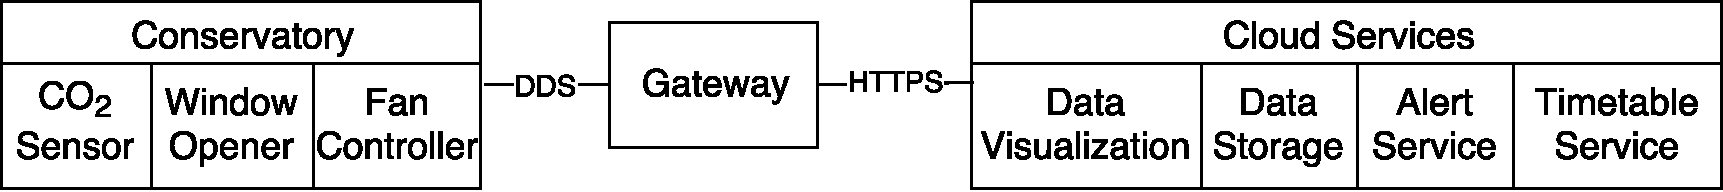
\includegraphics{fig/architecture.pdf}
			}
			\caption{The architecture of the CPS.}
			\label{fig:architecture}
		\end{figure}

	\subsection{Conservatory}
	\label{sec:conservatory}
	The \textbf{conservatory}, as presented above, is the physical entity where the concentration of carbon-dioxide needs to be controlled. It has a single fan as well as two windows, which can be accessed using the fan controller and the window handling engine actuators. The CO$_2$ concentration level can be sensed using the carbon-dioxide sensor. In this task we do not have to set or handle the conservatory physically. Instead, the sensing and actuating activities can be accessed via well-defined Data Distribution Service (DDS)\footnote{http://www.omg.org/spec/DDS/1.4} commands. The data structure of the commands is described by the following IDL\footnote{http://www.corba.org/omg\_idl.htm} snippet.
	\begin{lstlisting}[
		basicstyle=\small, %or \small or \footnotesize etc.
	]
struct Conservatory{
  string ID; //@key
  double Value;
  long TimeStamp;
};
	\end{lstlisting}
	
	Table \ref{tab:conservatory-dds} summarizes the valid DDS commands that can be used for communication with the conservatory on the DDS channel.
	
	\begin{mytable}{Valid DDS commands of the conservatory.}{conservatory-dds}{|cccc|}
		\hline
		\textbf{Topic} & \textbf{Read/Written} & \textbf{ID} & \textbf{Possible Values} \\ \hline \hline
	\end{mytable}
	
	\subsection{Gateway}
	
	The task of the \textbf{gateway} is to control the carbon-dioxide level of the conservatory using its sensor and actuators. The communication between the conservatory and the gateway is based on DDS \ref{sec:conservatory}. Furthermore, the gateway utilizes cloud services -- via the HTTPS protocol -- to ensure the quality of the controlling service.
	
	The gateway periodically samples the CO$_2$ concentration level of the conservatory and takes further actions based on the received value. The activity is represented in Figure \ref{fig:activity} using an activity diagram.
		
	\begin{figure}[h!]
		\center
		\resizebox{140mm}{!}{
			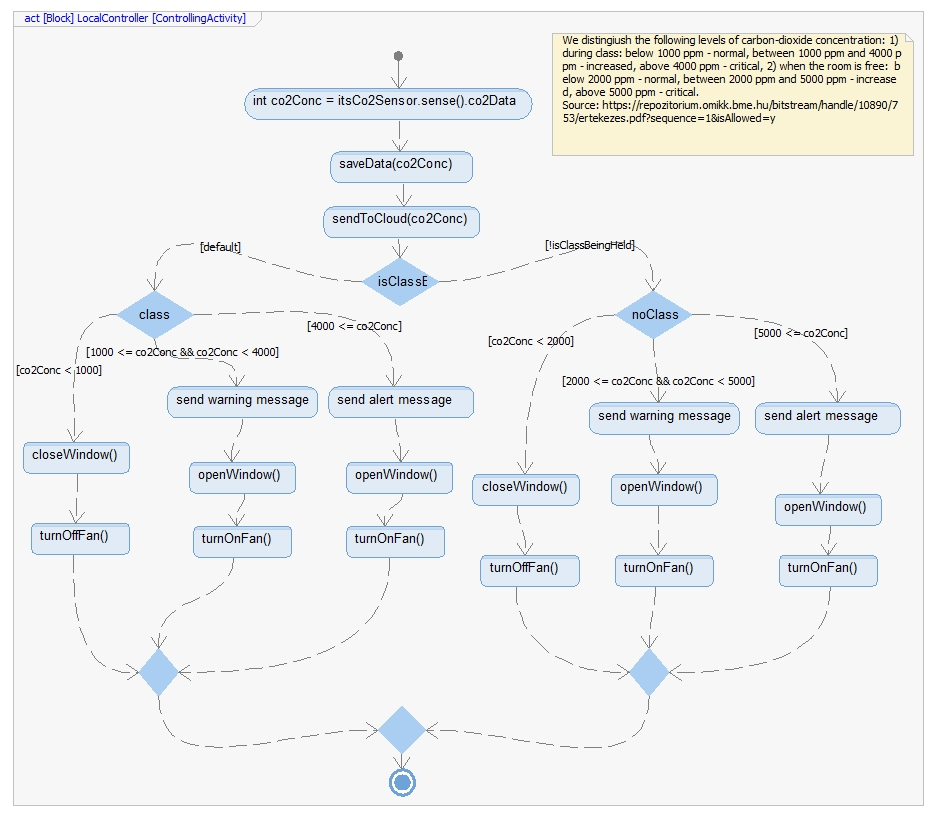
\includegraphics{fig/activity.jpg}
		}
		\caption{The activity diagram describing the periodic activity of the gateway.}
		\label{fig:activity}
	\end{figure}
	
	\subsection{Cloud Services}
	The \textbf{cloud services}, apart from the timetable service, are tightly integrated with each other. The data coming to the cloud is stored on persistent containers. Also, the visualization of stored data is supported. Furthermore, if certain values of the incoming data are too high, alerts (in the form of e-mails) can be sent. Finally, the timetable service holds information about the lessons taking place in the room represented by the conservatory.
	
	The timetable service is our custom implementation, whereas the other cloud services are provided by commercial cloud service providers.
	
	\subsubsection{Timetable Service}
	
	\subsubsection{Data and Alert Services}
	
	Figure \ref{fig:cloud} depicts the integration of the cloud services in Microsoft Azure.
		
	\begin{figure}[h!]
		\center
		\resizebox{125mm}{!}{
			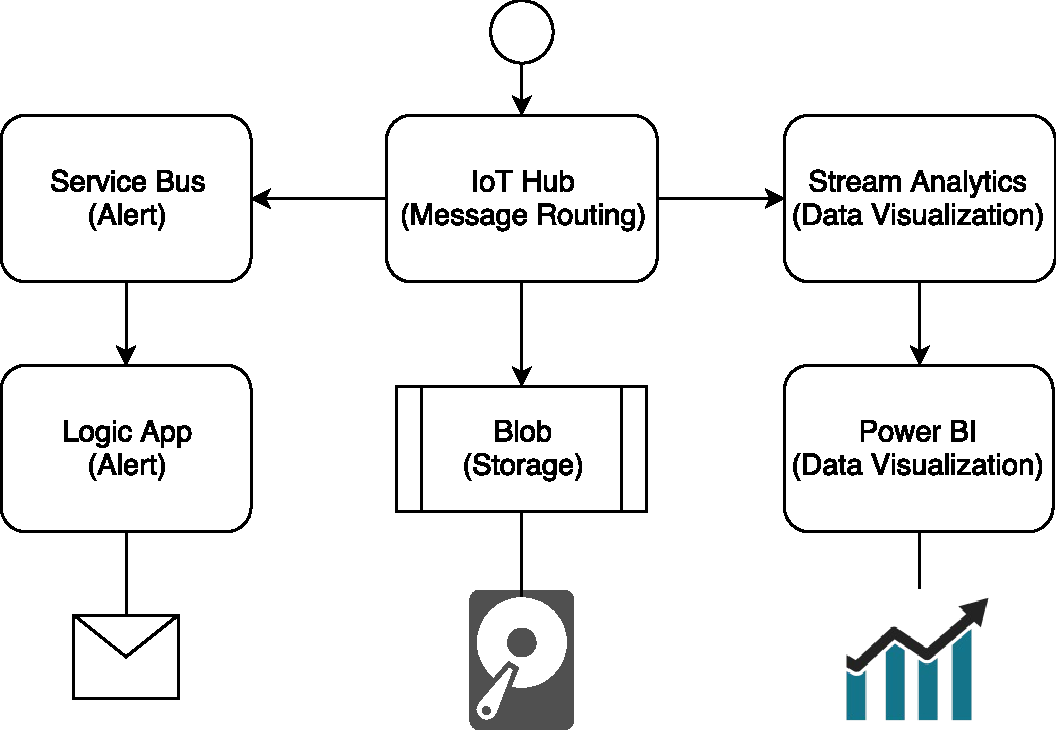
\includegraphics{fig/cloud.pdf}
		}
		\caption{The data flow in the cloud.}
		\label{fig:cloud}
	\end{figure}
	
	Each message transmitted to the cloud is first processed by the IoT Hub. This is the central element in the cloud. It is 		capable of routing incoming messages to other service nodes based on certain properties. The additional services are as follows.
	 \begin{itemize}
	 	\item Each message is transferred to the blob and saved (persistent storage).
		\item Each message is transfered to the stream analytics service that sends the data to the Power BI visualization service.
	 	\item If the alert property of a message is \textsl{true}, then a message is transmitted to the alert service bus. The service bus stores the messages in its queue and forwards them one-by-one to the alert logical app. The logical app is responsible for sending e-mails to the specified addresses.
	 \end{itemize}
	
	\section{Implementation}
	\label{sec:implementation}
%	Figure \ref{fig:architecture} depicts the architecture of the implemented CPS. As can be seen, the system consists of three bigger blocks: the conservatory, a gateway and the cloud. 
%	
%	\begin{figure}[h!]
%		\center
%		\resizebox{140mm}{!}{
%			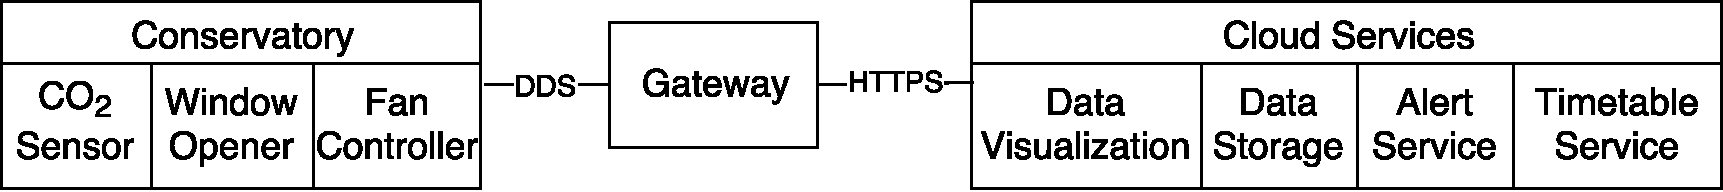
\includegraphics{fig/architecture.pdf}
%		}
%		\caption{The architecture of the CPS.}
%		\label{fig:architecture}
%	\end{figure}
%
%	The \textbf{conservatory} is the physical entity where the concentration of carbon-dioxide needs to be controlled. It has a single fan, which can be used to circulate the air, as well as two windows, which can be opened and closed. Regarding sensors and actuators, the conservatory contains a carbon-dioxide sensor in addition to the two window openers and a fan controller.
%	
%	The job of the \textbf{gateway} is to control the carbon-dioxide level of the conservatory using its sensor and actuators. The communication between the conservatory and the gateway is based on DDS. Furthermore, the gateway utilizes cloud services (via the HTTPS protocol) to ensure the quality of the controlling service.
%	
%	The \textbf{cloud services} (apart from the timetable service) are tightly integrated with each other. The data coming to the cloud is stored on persistent containers. Also, incoming data can be visualized. Furthermore, if certain values of the incoming data are too high, alerts can be sent. Finally, the timetable service holds information about the lessons taking place in the room represented by the conservatory.
%	
%	\section{Gateway Functionalities}
%	This section introduces the most important functionalities of the gateway on a lower abstraction level. All gateway functionalities have been implemented in Java 8.
%	
%	After the gateway is initiated, it initializes the DDS infrastructure. It has a single reader entity, which reads the carbon-dioxide concentration on the particular topic where the gas sensor of the conservatory publishes its data. Additionally, it has a writer entity responsible for publishing commands on the corresponding topic, which control the window opener and fan controller of the conservatory in accordance with the sensed carbon-dioxide concentration level.
%	
%	The handling of incoming data is implemented in accordance with the activity diagram presented in the system design (see Figure \ref{fig:activity}).
%	
%	\begin{figure}[h!]
%		\center
%		\resizebox{140mm}{!}{
%			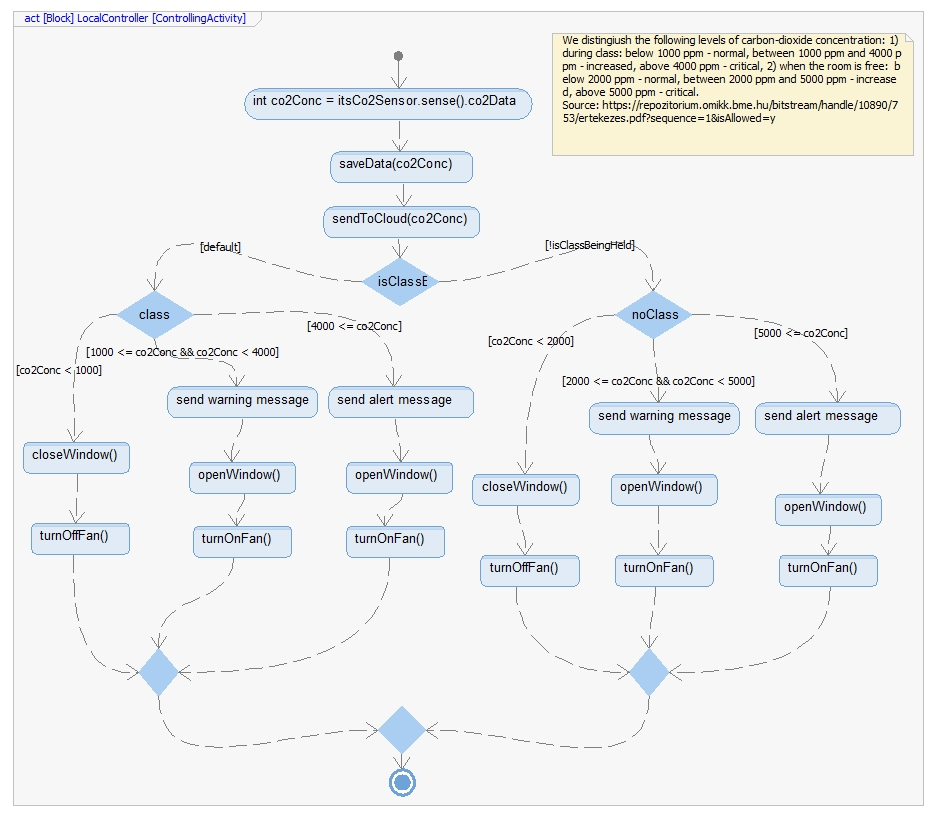
\includegraphics{fig/activity.jpg}
%		}
%		\caption{The activity diagram of LocalController.}
%		\label{fig:activity}
%	\end{figure}
%
%	The logic reacts differently based on whether there is a lesson taking place in the room in the particular moment or not. To get this information the gateway communicates with the timetable service periodically (every minute by default) and stores the answer. This communication takes place via a well-defined REST API:
%	\begin{itemize}
%		\item HTTP verb: GET.
%		\item URL where the request needs to be sent:		
%		http://152.66.181.77:8080/ \\ hu.bme.mit.cps.timetable/timetable/lesson.		
%		\item Answer: a JSON structure containing a \textsl{date} field with the date of the reply and a \textsl{lesson} field indicating whether there is a lesson held at the particular moment (true/false).
%		\begin{lstlisting}[
%		basicstyle=\small, %or \small or \footnotesize etc.
%		]
%{"date":"Dec 11, 2017 10:15:00 PM", "lesson":"true"}
%		\end{lstlisting}
%	\end{itemize}
%
%	Furthermore, the gateway communicates with the cloud each time it receives data from the conservatory. This is achieved by using the \textsl{DeviceClient} class of the Azure Development Kit.
%	Each message transmitted to the cloud conforms to the following JSON format.
%	\begin{lstlisting}[
%		basicstyle=\small, %or \small or \footnotesize etc.
%	]
%{"id":"messageId","value":95.39,"timeStamp":925971383,
%"comment":"critical"}
%	\end{lstlisting}
%	
%	\section{Cloud Services}
%	This section introduces the cloud services on a lower abstraction level. The timetable has been implemented by the author, whereas the other services are based on the commercial services of Microsoft Azure\footnote{https://azure.microsoft.com/}.
%	
%	\subsection{Timetable Service}
%	The timetable service is based on the Maven WildFly 10.x server. On each request, it reads a local file that stores data about the reservations of the presented room. The data is stored in accordance with the following JSON structure:
%	\begin{lstlisting}[
%	basicstyle=\small, %or \small or \footnotesize etc.
%	]
%{"lessons":[
%{"lessonName":"CPS","beginning":"Dec 11, 2017 10:15:00 PM",
%"end":"Dec 11, 2017 11:45:00 PM"},
%{"lessonName":"SWSV","beginning":"Dec 11, 2017 12:15:00 PM",
%"end":"Dec 11, 2017 13:45:00 PM"}
%]}
%	\end{lstlisting}
%	As can be seen, the entries are stored in a list (\textsl{lessons}). An entry has the following fields: \textsl{lessonName} is a string value, whereas the \textsl{beginning} and \textsl{end} are two date value.
%	
%	The server logic is simple. When a request arrives, it checks whether there is an entry defining a lesson in the particular moment. Also, the server is responsible for deleting old entries to save storage space.
%	\subsection{Azure Services}
%	Figure \ref{fig:cloud} depicts the integration of the cloud services in Microsoft Azure.
%	
%	\begin{figure}[h!]
%		\center
%		\resizebox{125mm}{!}{
%			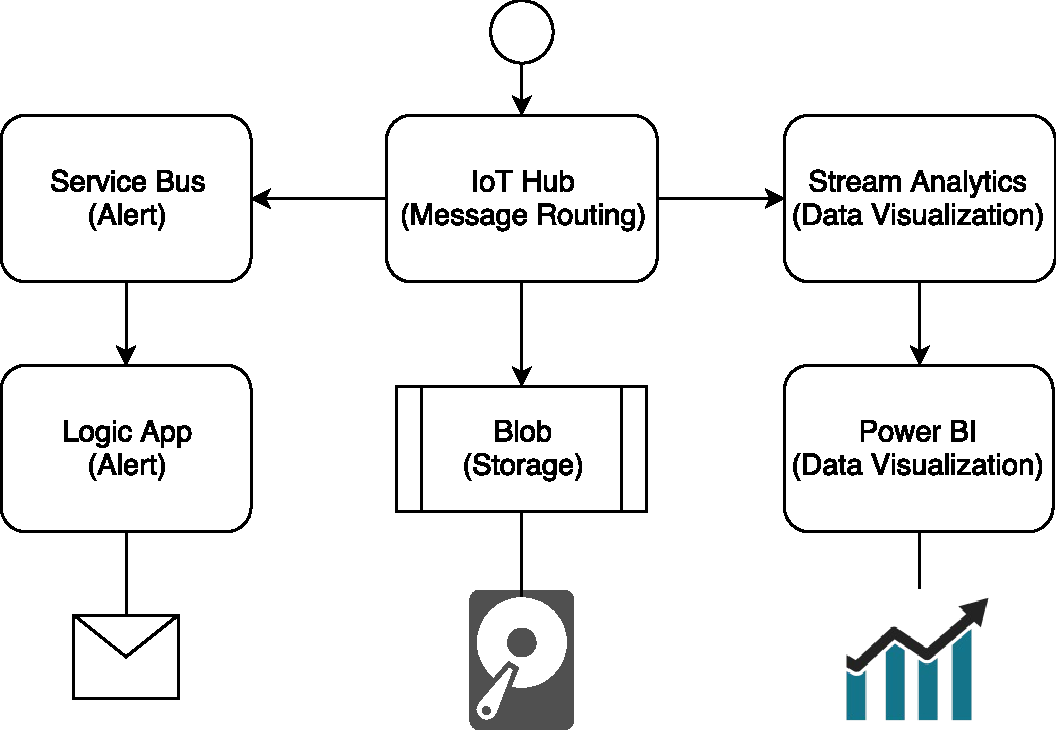
\includegraphics{fig/cloud.pdf}
%		}
%		\caption{The data flow in the cloud.}
%		\label{fig:cloud}
%	\end{figure}
%
%	 Each message transmitted to the cloud is first processed by the IoT Hub. This is the central element in the cloud. It is capable of routing incoming messages to other service nodes based on certain properties. The additional services are as follows.
%	 \begin{itemize}
%	 	\item Each message is transferred to the blob and saved (persistent storage).
%	 	\item Each message is transfered to the stream analytics service that sends the data to the Power BI visualization service.
%	 	\item If the alert property of a message is \textsl{true}, then a message is transmitted to the alert service bus. The service bus stores the messages in its queue and forwards them one-by-one to the alert logical app. The logical app is responsible for sending e-mails to the specified addresses.
%	 \end{itemize}
	
	\section{Conclusion}
	
	
\end{document}